\chapter{Landasan Teori}
    \section{Sebuah Tabel}
        \Blindtext[1][1]
        \begin{table}[h]
            \centering
            \caption{Contoh Tabel}
            \begin{tabular}{|l|l|l|}
                \hline
                Wiramaswara & Lalalala & Widya  \\ \hline
                Lelelele    & Lalalala & Lalala \\ \hline
            \end{tabular}
        \end{table}
        \Blindtext[1][1]
    \section{Sebuah Gambar}
        \Blindtext[1][1]
        \begin{figure}[h]
            \centering
            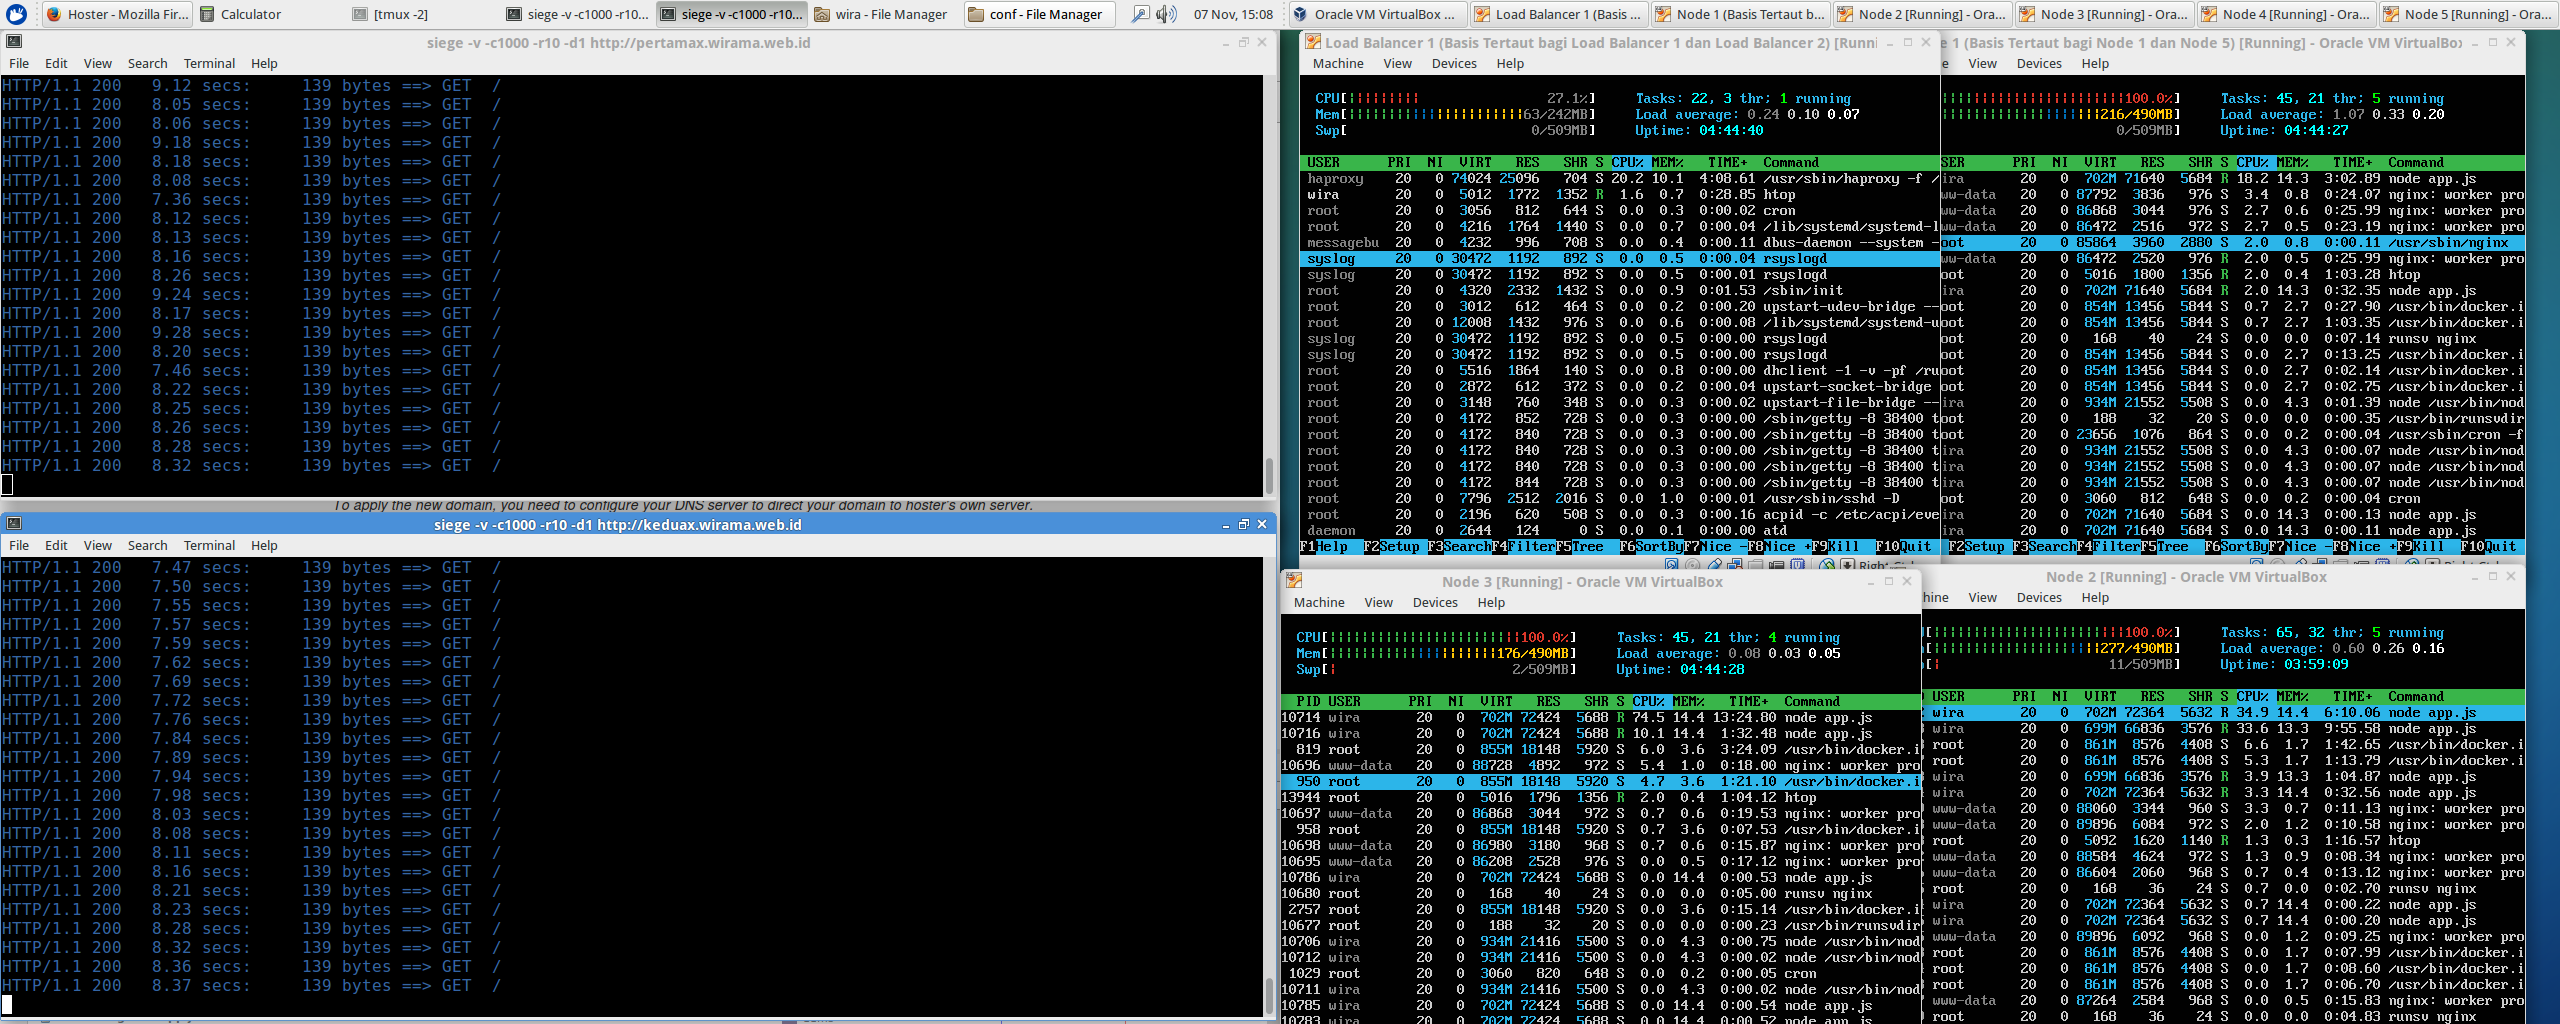
\includegraphics[width=1\textwidth]{tes.png}
            \caption{Coba gambar}
            \label{fig:testGambar}
        \end{figure}
    \section{Sebuah Kode}
        \begin{figure}[h]
            \begin{minted}{csharp}
string title = "This is a Unicode π in the sky"
const double pi = 3.1415926535
            \end{minted}
            \caption{Sebuah kode}
        \end{figure}
    \cleardoublepage
